\section{Language Models - Benchmarks and Leaderboards}\label{sec:b}


\epigraph{I often say that when you can measure what you are speaking about, and express it in numbers, you know something about it; but when you cannot measure it, when you cannot express it in numbers, your knowledge is of a meagre and unsatisfactory kind; it may be the beginning of knowledge, but you have scarcely, in your thoughts, advanced to the stage of science, whatever the matter may be.}{\textit{William Thomson, 1st Baron Kelvin}}

In many situations in our lives, we face the problem of measuring. Sometimes is the temperature of the oven, sometimes it is the quality of a \gls{LLM}. It is often said that if you can't measure something, you can't improve or control it, which is mostly true, if you miss the right temperature you will ruin your meal and if you don't know how an \gls{LLM} behaves you will get nonsense from it. 
However, depending on the problem at hand, measuring something can also become a problem. If we are designing ovens and we focus solely on controlling the oven temperature and forget that food needs to fit in you will get a wonderful temperature control that wont help you make a cake, or in the case of \glspl{LLM}, you will get outstanding scores that wont actually mean anything. This problem was conceptualized by Charles Goodhart, "When a measure becomes a target, it ceases to be a good measure"~\cite{strathern1997improving}, meaning that over focusing on some measurements results in failure.
In the engineering world live in a constant fight between these two concepts, trying to measure something and trying not to get blinded by the resulting metrics. In the case of ovens we are somewhat above this problem and we know whats important to build them and make great food, on the case of \glspl{LLM}, we are not there yet.


Through the time, and more specifically in the field of engineering, having a \gls{CTF} helped set the objectives and measure the improvements of a given field, let it be machine translation, hand-written character recognition, or any task. A \gls{CTF} is normally composed of~\cite{donoho201750}:
\begin{itemize}
    \item A public dataset, feature measurements and labels.
    \item A set of participants, engaged in the task of predicting labels.
    \item A scoring referee, to which competitors can submit their work for evaluation.
\end{itemize}
The field of \gls{ML} grew very used to these kinds of setups to track and guide the advancement of research, and many important competitions were created following these patterns, for example using EMNIST~\cite{cohen2017emnist} for hand-written number recognition or SuperGLUE~\cite{wang2019superglue} for text understanding.

As we know, the \glspl{LLM} are \gls{ML} models and as such the way that we measure them is by mean of \glspl{CTF}. An special quality of the \glspl{LLM} is that they are not used for a single thing and these makes them a little harder to measure. For example, in the past it was enough for a vision model to achieve a great score in the MNIST dataset to revolutionize the field of \gls{ML}, like AlexNet~\cite{krizhevsky2012imagenet} did. Today \glspl{LLM} need to past several of these tests to create impact. It's not enough for \glspl{LLM} to excel at a single \gls{CTF}, a \gls{LLM} needs to be good at a large variety of them. Now the question is: Which of them? There are many \glspl{CTF} from where to choose, testing all of them is expensive and making sense of all the generated numbers is difficult. To solve this the scientific community came up with collections of \glspl{CTF} that are organized into \emph{leaderboards} or \emph{benchmarks}, being the most publicly known the \gls{HELM}~\cite{liang_holistic_2023} and \gls{LMEH}~\cite{eval-harness}.

At this point, we can see that in order to measure the quality of a \gls{LLM} is not a straightforward thing. Lots of discretional choices are made in the process of selecting a benchmark to use (like, what I want to know about the \gls{LLM}, or what is its application). Also, the selected benchmark is built upon many assumptions around how the different \glspl{CTF} reflect the various characteristics of a \gls{LLM}. Finally, each of these \glspl{CTF} are constructed on datasets that have other assumption or limitations (like, they are built from whats available and not form what they need sample to measure something~\cite{raji2021ai}).

We can see how measuring a \gls{LLM} is far more complicated that measuring the oven temperature, and how fragile and opinionated is the construction of the benchmarks or leaderboards, as opposed to setting the right temperature to bake a cake~\footnote{We acknowledge our lack of experience in baking cakes and apologize for this oversimplification.}. However, as Lord Kelvin points out, we need to measure something in order to know something even when it means that we are accepting lots of assumptions.



\subsection{Language Model Evaluation Harness}

Today there are a large number of benchmarks that can be implemented to describe the quality of a \gls{LLM}. Their number grows constantly, so we wont try to mention all of them. In this section we will focus on a single one of them, the \gls{LMEH}.
We choose to use this framework due to be the one used to compute the \gls{HF} Open \gls{LLM} leaderboard~\cite{open-llm-leaderboard}, shown in figure \ref{fig:hf_leaderboard}. This leaderboard is usually referenced when comparing different language models and since the Pocket Network will be composed of mostly open models, it is an easy choice that will provide the Pocket \gls{MLTB} with a direct comparison.

\begin{figure}[H]
    \centering
    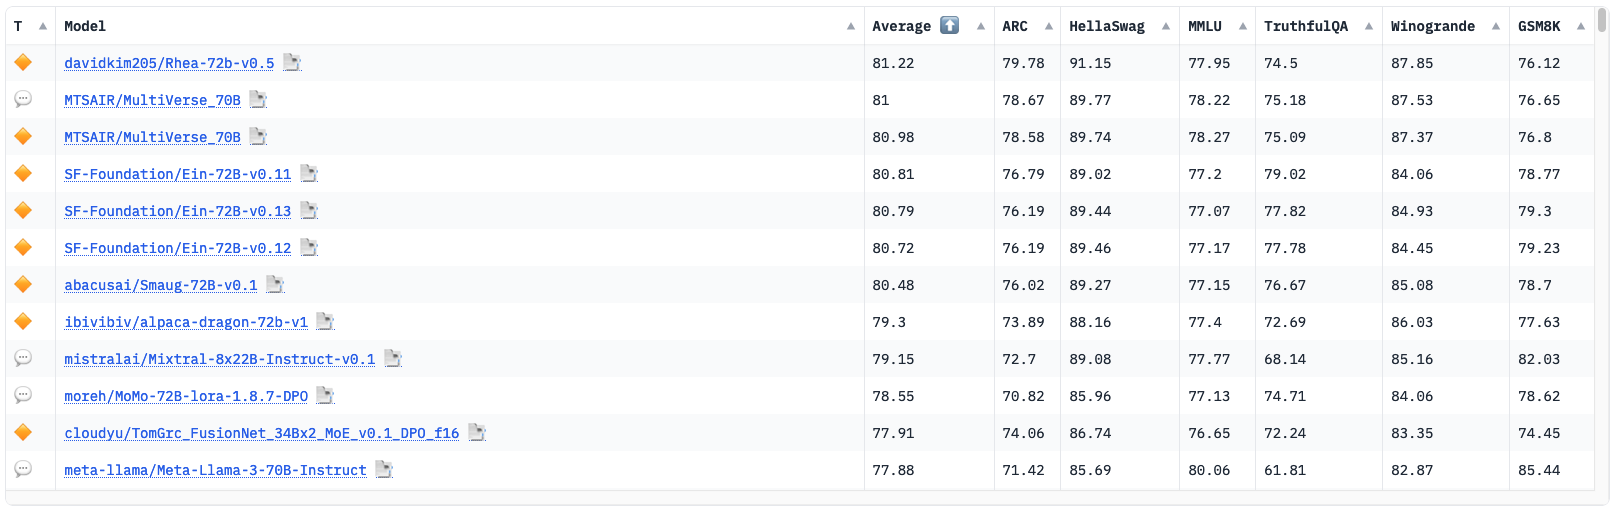
\includegraphics[width=0.95\textwidth]{hf_leaderboard.png}
    \caption{Screenshot of the Hugging Face Open LLM leaderboard (\url{https://huggingface.co/spaces/HuggingFaceH4/open_llm_leaderboard}) taken on 2024-04-25.}
    \label{fig:hf_leaderboard}
\end{figure}

The \gls{LMEH} is composed of many different \glspl{CTF} built upon many datasets~\footnote{\gls{LMEH} supports $\approx$90 datasets at the time of writing} and each of them with one or more associated metrics. The pair of dataset-metrics makes up a \emph{task}, and a leaderboard is composed of many tasks. The one that we want to reproduce initially for the Pocket Network is the Open \gls{LLM} leaderboard from \gls{HF} which is based on many paris of task-dataset, organized in 6 groups:
\begin{itemize}
    \item AI2 Reasoning Challenge~\cite{clark2018think} : Natural questions from grade-school science created for testing humans.
    \item HellaSwag~\cite{zellers2019hellaswag} : Sentence completion tasks that are trivial to humans, designed to test model's commonsense.
    \item MMLU~\cite{hendrycks2020measuring} : Multiple choice questions on more than 57 tasks, including elementary mathematics, US history, computer science, law, and more.
    \item TruthfulQA~\cite{lin2021truthfulqa} : Questions designed to test common human misconceptions on 38 categories, including health, law, finance and politics.
    \item Winogrande~\cite{sakaguchi2019adversarial} : A set of 44000 expert-created questions to test commonsense reasoning, created via crowdsourcing.
    \item GSM8k~\cite{cobbe2021training} : A set of 8500 grade school math problems written in a linguistically diverse way.
\end{itemize}

The calculation of the scores in each of these areas varies depending on the task, but there are three main ways of getting an score (for these or any other tasks):
\begin{itemize}
    \item Accuracy: The model is given a prompt and the generated text is compared to the expected answer and the number of correct matches is used. The comparison for a correct answer can be using an exact match or near matches, for example, if you ask "who was the first person in the moon?" the answer should be "Neil Armstrong", or "Neil Alden Armstrong" or "Armstrong, Neil A." and so on. Also, used in most multiple choise tests, the answer of the \gls{LLM} can be chosen by presenting each question-answer pair to the model and selecting that with the highest generation probability~\footnote{by means of the tokens probabilities, also calculated by the \gls{LLM}.}.
    \item Perplexity: In this case the "surprise"  of the model is calculated for each answer. Given a prompt, the probability that the model would produce that prompt is calculated. A higher perplexity means that the model is less likely to produce a given prompt. So, if a given question-answer pair has a high perplexity it means that the model is not confident on this answer (usually used to  test the correct answer).
    \item Others: There are also metrics specific to compare models outputs, like BLEU~\cite{papineni2002bleu} or ROUGE~\cite{lin2004rouge} that will provide a value of how much text pieces relate (useful to compare summarization tasks).
\end{itemize}

In conclusion, a leaderboard like the one in \gls{HF} is nothing more than a collection of metrics that were calculated based on known tasks (datasets), so, in order to reproduce it we only need to execute a set of tasks on the nodes in the Pocket Network and reconstruct the leaderboard using the \gls{LMEH} framework (which is not so easy, as we will see section~\ref{sec:c}). 


\subsection{Leaderboards Weaknesses}

Until now we described the how a \gls{LLM} is measured and what are the accepted ways of grouping and presenting the scores. However there is a big issue around all this subject that is not often talk about, which is the validity of them.

The selected tasks used in the \gls{HF} leaderboard are not justified using a developed taxonomy like the one proposed in \gls{HELM}, they seem to respond to simpler motivations, focused on providing enough task diversity (covering, language, reasoning, knowledge and math) using the available and relevant datasets that are interesting to the community and relevant to real-world use cases. This last point is a key issue, the relevance of them to real-world use cases.

When we described the metrics used in the \gls{HF} leaderboard we talked about 6 groups of tasks, each of them specialized in different areas of interest. If we go deeper into the selected tasks, we will find that instead of 6 metrics (the columns shown in figure \ref{fig:hf_leaderboard}), around 60 metrics are calculated and then they are averaged into categories (for example, for the MMLU score, the score for law knowledge is averaged with math). Moreover, many people only look at the average, which is an average of averages of wildly different things. 
Now the question seems obvious, what does this mean? are these leaderboards even useful for something?

The world of \gls{ML} faces this problem since a while, it seem to have fallen victim of its own thirst for achieving the next \gls{SOTA} and revive the history of AlexNet. This subject is really vast and we wont pretend to cover it here~\footnote{For a comprehensive read on this subject we recommend the following works:~\cite{nityasya2023scientific}~\cite{chollet2019measure}~\cite{raji2021ai}}, we only want to highlight the current limitations and how the Pocket Network can help.

A key missing piece in relating scores to actual usefulness is the feedback from users, not only prompt-based feedback like the one we give the various \gls{LLM} chat bots when they kindly ask for it, but market feedback. Going back to the example of ovens, how did we got so good at building ovens? We could argue that it was in part a selection process where those ovens that did not have the correct balance between temperature control and cavity size were not selected by buyers and they disappeared. The buyer probably were unaware of the many metrics that a particular oven had and just selected the oven that fitted their needs. In the same spirit we can believe that the Pocket Network could be the missing piece between the leaderboards and the users, the free market place were models come to find users and users could freely change from one model to another until they find the best one. This usage data, correlated with a correlated leaderboard (a set of \glspl{CTF}) can be of great utility to guide the development of new models tailored for real-world use cases. In the end we might finally get a \gls{LLM} as reliable as our good old oven.